\subsection{E6: a scalability stress test, not a scaling law}
\label{sec:res-e6}

This campaign was designed to measure how the recovery threshold scales, and it does not have
the resolution to do that. We report it for what it does establish --- that the measurement
itself runs at a width and feature count where the code cannot be materialised --- and withdraw
the scaling-law reading.

Scaling to $d=\EsixDmax$ at $F=\EsixFmax$ features lets the recovery threshold be traced over
a factor of eight in width (Table~\ref{tab:e6}, Fig.~\ref{fig:e6}). On the grid, $s_{95}$ grows
from \EsixOneTwoEightSNF{} at $d=128$ to \EsixOneZeroTwoFourSNF{} at $d=\EsixDmax$.

That grid statistic needs care, because it floors the crossing and floors it unevenly. The
true 95\% crossing lies between grid points, and the gap is proportionally largest where the
transition is sharp relative to the spacing --- at $d=128$ the interpolated crossing is
\EsixInterpOneTwoEight{} against a reported 1. Interpolating instead of flooring changes the
headline: growth over the sweep falls from \EsixGrowthGrid{} to \EsixGrowthInterp, against
\EsixGrowthPredicted{} for an exact $d/\ln d$ law. The floored figure therefore overstates the
growth by roughly a third, purely as an artefact of the grid, and we quote the interpolated
values from here on.

Four widths then cannot identify a law. On the interpolated crossings a one-parameter fit of
$s_{95}=c\,d/\ln d$ gives $c=\EsixInterpC$ with $R^2=\EsixInterpRsqLog$ over
\EsixFitPoints{} points, but a plain linear law $c\,d$ reaches $R^2=\EsixInterpRsqLin$ and
$c\,d/\ln^2 d$ reaches $R^2=\EsixInterpRsqLogSq$ on the same four points. The three are
indistinguishable on this evidence, the base of the logarithm is not identifiable at all, and we
therefore claim no scaling law --- neither for $d/\ln d$ nor against it. A previous version of
this work drew a $d/(16\ln d)$ reference curve here; it has been withdrawn, because its constant
is inherited from the earlier literature rather than derived anywhere in this work, and because
it sat \emph{above} the measured thresholds at every width and so was not the conservative
reference its form suggests. Corollary~\ref{cor:separation} fixes only the shape
$s\le c\,d/\log d$, for an unspecified universal $c$.

A second qualification. $s_{95}$ is a point estimate: at $d=\EsixDmax$ the campaign runs
\EsixOneZeroTwoFourTrials{} trials, so even a flawless \EsixOneZeroTwoFourTrials{}-for-%
\EsixOneZeroTwoFourTrials{} result gives a Wilson lower bound of only
\EsixTopBestWilsonLow. No sparsity at that width can be certified at the 95\% level with 95\%
confidence on this budget; the reported thresholds are best estimates, and a claim at
confidence would need more trials.

The whole campaign took \DurEsixMin{} minutes on CPU, with $d=\EsixDmax$ accounting for
\EsixOneZeroTwoFourDurationMin{} of them over \EsixOneZeroTwoFourTrials{} trials. Materialising
the code at that size would have required $4$~GB; the streaming implementation of
Algorithm~\ref{alg:ensemble} keeps the peak footprint proportional to $Bd$.

\begin{figure}[t]
\centering
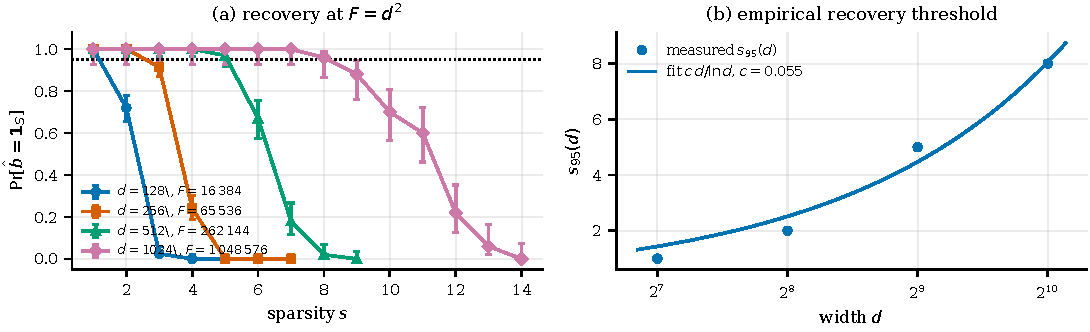
\includegraphics[width=\linewidth]{figures/fig4_scaling.pdf}
\caption{\textbf{Threshold recovery at quadratic feature load, up to $d=\EsixDmax$}
($F=\EsixFmax$). (a) Empirical exact-recovery probability with Wilson $95\%$ intervals; a fresh
random code is drawn per trial. (b) The empirical threshold $s_{95}(d)$ with the fitted
$c\,d/\ln d$ curve shown as a fit only: four widths do not distinguish it from $c\,d$ or from
$c\,d/\ln^2d$, and no scaling law is claimed. Generated by
\code{scripts/make\_figures.py} from \code{results/e6}.}
\label{fig:e6}
\end{figure}

\begin{table}[t]
\centering
\caption{E6: recovery threshold and measured cost by width.}
\label{tab:e6}
\small
% Generated by scripts/make_tables.py from results/. Do not edit by hand.
\begin{tabular}{rrrrrr}
\toprule
$d$ & $F=d^2$ & trials & $s_{95}$ & $d/(16\ln d)$ & wall clock (min) \\
\midrule
128 & 16\,384 & 200 & 1 & 1.65 & 1.5 \\
256 & 65\,536 & 200 & 2 & 2.89 & 2.2 \\
512 & 262\,144 & 100 & 5 & 5.13 & 4.9 \\
1024 & 1\,048\,576 & 50 & 8 & 9.23 & 21.3 \\
\bottomrule
\end{tabular}

\end{table}

